\section{Materials and Methods}

\subsection{Study area and monitoring sites}
The study area encompasses multiple rapidly urbanizing and industrializing airsheds across India. Specifically, the framework is trained and evaluated using data from major cities including Delhi, Kolkata, Hyderabad, Ahmedabad, Lucknow, and Patna. These cities represent distinct geographical and meteorological conditions, ranging from the landlocked, highly polluted Indo-Gangetic Plain (Delhi, Lucknow, Patna) to coastal and central-peninsular climates (Kolkata, Hyderabad), as well as semi-arid industrial hubs (Ahmedabad). 

Table \ref{tab:stations} summarizes the specific CAAQMS monitoring data utilized in this study, detailing their respective cities, settings, valid hourly records, and data split allocation. Maninagar, although located in Ahmedabad, was designated as the validation station to provide an in-domain stopping criterion prior to final evaluation on the completely held-out cities.

\begin{table}[h]
\centering
\caption{Summary of continuous ambient air quality monitoring stations (CAAQMS) utilized in this study, including setting and data split allocation.}
\label{tab:stations}
\resizebox{\textwidth}{!}{
\begin{tabular}{lllc}
\toprule
\textbf{City/Station} & \textbf{Setting} & \textbf{Valid Hours} & \textbf{Split Allocation} \\
\midrule
Delhi & Urban Background & 16,595 & Train \\
Kolkata & Urban Industrial & 15,283 & Train \\
Hyderabad & Urban Background & 14,542 & Train \\
Ahmedabad & Urban Industrial & 13,633 & Train \\
Maninagar & Urban Background & 14,637 & Validation (In-domain) \\
Lucknow & Urban Background & 10,930 & Test (Zero-Shot) \\
Patna & Urban Background & 15,229 & Test (Zero-Shot) \\
\bottomrule
\end{tabular}
}
\end{table}

\subsection{Data sources}

\subsubsection{CPCB ground measurements}
The primary target variable for the predictive models is the hourly surface-level $PM_{2.5}$ concentration, obtained from the Central Pollution Control Board (CPCB) CAAQMS portal for the period 2019--2023. To ensure data integrity, quantitative quality control was applied (summarized in Table \ref{tab:qc_stats}). Hourly records with negative concentrations, duplicate timestamps, invalid timestamps, and prolonged repeated-value runs (sensor freezes, defined as $\ge 6$ consecutive identical hours) were excluded. Short gaps of $\le 3$ consecutive hours were interpolated using linear time-interpolation only to maintain input-sequence continuity; crucially, interpolated target observations were excluded from final test-metric calculations. Whether interpolated values were used as Stage 2 input features was strictly limited to these short gaps to avoid introducing synthetic artifacts.

\begin{table}[h]
\centering
\caption{Quantitative summary of the data quality control pipeline.}
\label{tab:qc_stats}
\resizebox{\textwidth}{!}{
\begin{tabular}{lcccccc}
\toprule
\textbf{Station} & \textbf{Raw Records} & \textbf{Negatives Removed} & \textbf{Duplicates Removed} & \textbf{Freezes Removed} & \textbf{Interpolated Hours} & \textbf{Valid Observed Hours} \\
\midrule
Delhi & 16,842 & 56 & 0 & 80 & 1,079 & 16,595 \\
Kolkata & 15,342 & 52 & 0 & 0 & 621 & 15,283 \\
Hyderabad & 14,784 & 5 & 0 & 132 & 803 & 14,542 \\
Ahmedabad & 13,825 & 142 & 0 & 24 & 589 & 13,633 \\
Maninagar & 14,831 & 141 & 0 & 12 & 687 & 14,637 \\
Lucknow & 11,053 & 108 & 0 & 0 & 263 & 10,930 \\
Patna & 15,533 & 200 & 0 & 26 & 1,015 & 15,229 \\
\bottomrule
\end{tabular}
}
\end{table}

\subsubsection{Meteorological data}
High-resolution hourly meteorological data were sourced from the Open-Meteo historical ERA5 reanalysis archive (0.25$^\circ$ spatial resolution). The extracted variables include surface temperature ($^\circ$C), relative humidity (\%), surface pressure (hPa), precipitation (mm), wind speed (m/s), and wind direction ($^\circ$), as well as Planetary Boundary Layer Height (PBLH) which is provided directly by the ERA5 product. Data were extracted for the nearest grid cell corresponding to each station's coordinates, and UTC timestamps were rigorously converted to Indian Standard Time (IST). The present study evaluates the model under historical ERA5 meteorological inputs; operational forecast-mode performance using real-time predictive weather feeds remains to be assessed in future work.

\subsubsection{Satellite data (Sentinel-5P TROPOMI)}
To provide a spatial background for the unmonitored regions, satellite retrievals were integrated from the Sentinel-5P TROPOMI instrument via Google Earth Engine. Table \ref{tab:satellite} details the processing parameters for the specific GEE collections used. On days with missing satellite data due to severe cloud cover or collection gaps, the daily satellite features were masked, and the Stage-1 estimator relied primarily on daily meteorological and static features, ensuring the pipeline did not fail on overcast days.

\begin{table}[h]
\centering
\caption{Sentinel-5P TROPOMI data extraction and processing parameters.}
\label{tab:satellite}
\resizebox{\textwidth}{!}{
\begin{tabular}{lllll}
\toprule
\textbf{Feature} & \textbf{GEE Product Collection} & \textbf{Spatial aggregation} & \textbf{Quality filter} & \textbf{Temporal use} \\
\midrule
$NO_2$ VCD & COPERNICUS/S5P/NRTI/L3\_NO2 & Median in 5-km buffer & QA > 0.75 & Day $d$ \\
UVAI & COPERNICUS/S5P/NRTI/L3\_AER\_AI & Median in 5-km buffer & QA > 0.80 & Day $d$ \\
\bottomrule
\end{tabular}
}
\end{table}

\begin{figure}[htbp]
\centering
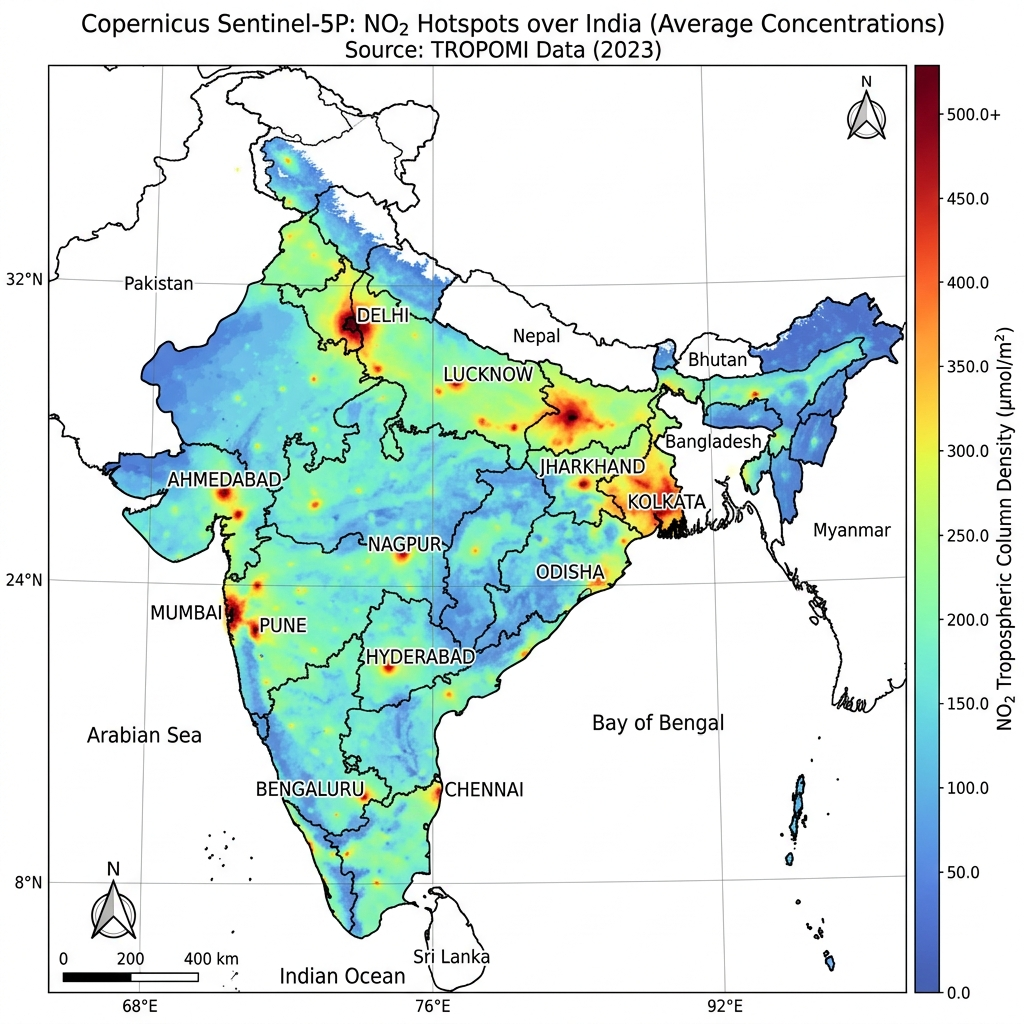
\includegraphics[width=0.8\textwidth]{figures/satellite_heatmap.png}
\caption{Visualization of Sentinel-5P spatial coverage over the Indian subcontinent, demonstrating baseline extraction capabilities.}
\label{fig:heatmap}
\end{figure}


\subsubsection{Static land-use features}
The spatial characteristics of each monitoring site were captured using static land-use features. NDVI and NDBI were derived as annual median composites within a 1-km buffer around each station, while elevation was extracted from a 30-m Digital Elevation Model (DEM) and population density from a gridded 1-km population product. These features provide localized context regarding emission potential and topology.

\subsection{Feature engineering}
To provide the model with features that represent physically plausible atmospheric mechanisms, raw meteorological variables were transformed:

\textbf{Trigonometric wind vectors:} Scalar wind speed and direction were converted into continuous orthogonal vectors ($U$ and $V$) representing East-West and North-South transport, eliminating the 360$^\circ$/0$^\circ$ discontinuity.

\textbf{Inverse Planetary Boundary Layer Height ($1/\text{PBLH}$):} To explicitly signal boundary layer collapse (e.g., during winter mornings), the inverse parameter was utilized. To prevent numerical instability when PBLH approaches zero, the feature was computed as $1/\max(\text{PBLH}, \epsilon)$, where $\epsilon = 10^{-5}$. To address skewness, the resulting inverse values were standardized via Z-score normalization prior to network ingestion.

\begin{figure}[htbp]
\centering
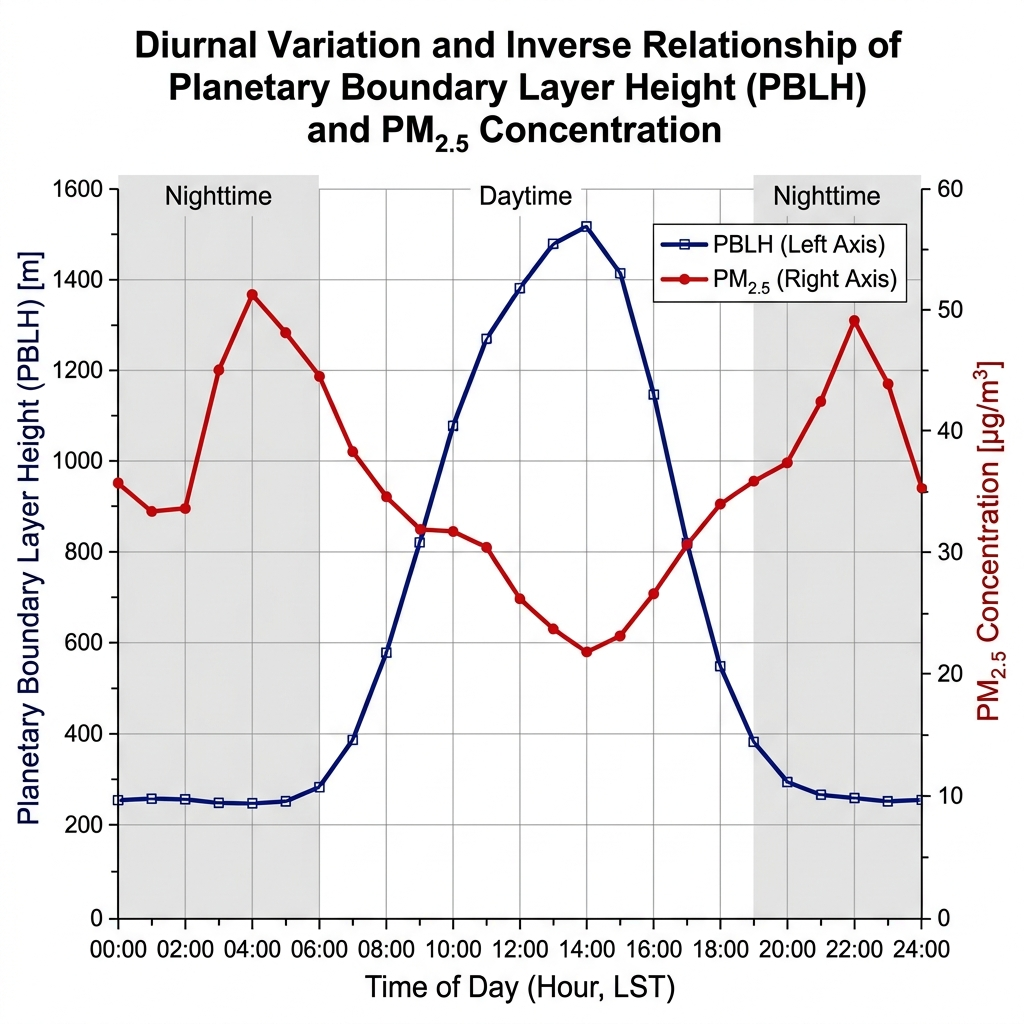
\includegraphics[width=0.8\textwidth]{figures/pblh_relationship.png}
\caption{The inverse relationship between Planetary Boundary Layer Height (PBLH) and $PM_{2.5}$ concentrations over a diurnal cycle.}
\label{fig:pblh}
\end{figure}


\textbf{Cyclic temporal encodings:} To preserve the continuity of diurnal and seasonal cycles, hour of the day ($h$) and month of the year ($m$) were transformed using sine and cosine encodings:
\begin{equation}
    h_{sin} = \sin\left(\frac{2\pi h}{24}\right), \quad h_{cos} = \cos\left(\frac{2\pi h}{24}\right)
\end{equation}
Equivalent equations were applied for the 12-month cycle.

\textbf{Upwind Fire Radiative Power (FRP):} As a proxy for episodic biomass burning, an upwind FRP feature was derived from NASA FIRMS MODIS/VIIRS thermal anomalies. It was computed by summing detected fire pixels within a 50-km radius, specifically restricting the sum to a 90$^\circ$ upwind wedge determined by the station's daily dominant wind direction. If no fires were detected, a default value of 0 was applied.

\subsection{Modeling framework}
A fundamental temporal mismatch exists when attempting to feed a singular daily satellite reading into an hourly predictive network. We resolve this via a Two-Stage Decoupled Architecture.


\begin{figure}[htbp]
\centering
\resizebox{\textwidth}{!}{
\begin{tikzpicture}[
    node distance = 1.2cm and 1.2cm,
    block/.style = {rectangle, draw, fill=blue!10, text width=3.2cm, align=center, rounded corners, minimum height=1.5cm, inner sep=0.2cm, font=\small},
    line/.style = {draw, -latex', thick}
]

% Nodes
\node [block] (sat) {Satellite Data\\(Sentinel-5P)};
\node [block, below=of sat] (met) {Meteorological Data\\(ERA5)};
\node [block, below=of met] (static) {Static Land-use\\(NDVI, DEM, Pop)};

\node [block, right=of met, fill=green!10, xshift=1cm] (stage1) {\textbf{Stage 1:}\\Daily Background\\Estimator (RF)};
\node [block, right=of stage1, fill=red!10, xshift=1cm] (stage2) {\textbf{Stage 2:}\\SpatioTemporal\\HybridNet};

\node [block, right=of stage2, fill=yellow!10, xshift=0.5cm] (output) {Hourly {2.5}$\\Predictions};

% Edges
\path [line] (sat) -| (stage1);
\path [line] (met) -- (stage1);
\path [line] (static) -| (stage1);

\path [line] (stage1) -- node[above, font=\footnotesize, align=center] {Daily\\Baseline} (stage2);

% Route met to stage 2 from below
\path [line] (met.south) -- ++(0,-0.6) -| (stage2.south) node[pos=0.25, below, font=\footnotesize, align=center] {Hourly Met Features};

\path [line] (stage2) -- (output);

\end{tikzpicture}
}
\caption{Block diagram of the proposed Two-Stage Decoupled Framework for virtual sensing.}
\label{fig:workflow}
\end{figure}

\subsubsection{Stage 1 – Daily background estimator}
Stage 1 acts as a daily background-scale estimator. A Random Forest model (configured with 100 trees and a maximum depth of 20) ingests the daily Sentinel-5P retrievals, historical full-day averaged meteorological data, and static land-use features. The Stage-1 target was explicitly defined as the arithmetic mean of the 24 observed hourly $PM_{2.5}$ values in the target window (requiring at least 18 valid hours per day). The predicted daily mean $PM_{2.5}$ serves as a conditioning variable and spatial magnitude reference for Stage 2.

\subsubsection{Stage 2 – SpatioTemporalHybridNet}
Stage 2 operates at an hourly resolution, transforming the static daily baseline into a dynamic 24-hour sequence. The target window corresponds to the same 24-hour day ($T_0$ to $T_{23}$) for which the daily satellite overpass provides a spatial background. Table \ref{tab:architecture} summarizes the network dimensions.

\begin{table}[h]
\centering
\caption{Architecture dimensions of the Stage-2 SpatioTemporalHybridNet.}
\label{tab:architecture}
\begin{tabular}{lll}
\toprule
\textbf{Module} & \textbf{Configuration} & \textbf{Output Dimension} \\
\midrule
Dynamic input & 24 timesteps $\times$ 11 dynamic features ($F_d$) & $24 \times 11$ \\
1D-CNN & 64 filters, kernel size 3 & $24 \times 64$ \\
BiLSTM & 2 layers, 128 hidden units per direction & $24 \times 256$ \\
Residual attention & Vector-valued softmax attention over sequence & $24 \times 256$ \\
Static/base fusion & Concatenation with 5 static features ($F_s$) + 1 baseline & $24 \times 262$ ($D$) \\
MLP & $262 \rightarrow 64 \rightarrow 1$ & $24 \times 1$ \\
Activation & Softplus (Yields positive ratios) & $24 \times 1$ \\
\bottomrule
\end{tabular}
\end{table}

\subsubsection{Multiplicative mapping}
The final physical concentration at hour $t$ is achieved via:
\begin{equation}
    \hat{y}_t = r_t \times \text{baseline}
\end{equation}
Note that the Softplus activation ensures strictly positive ratios ($r_t > 0$) but does not artificially bound them from above, nor does it strictly constrain the final 24-hour sequence mean to perfectly equal the Stage-1 baseline. The multiplicative parameterization was selected to factor the problem into daily magnitude and within-day modulation. We test this design against an additive alternative ($\hat{y}_t = b + \delta_t$, where $\delta_t$ is a dimensionless or concentration-based offset) in an ablation study.

\subsection{Training objective and optimization}
Although Mean Squared Error (MSE) assigns larger numerical penalties to large residuals, when high-concentration events are rare, minimizing average loss may still favor attenuated predictions. We therefore use target-frequency weighting to increase the training contribution of rare concentration bins.

The explicit formulation for the base Frequency-Weighted Mean Absolute Error ($\mathcal{L}_{fMAE}$) over a sequence of $N$ predictions is:
\begin{equation}
    \mathcal{L}_{fMAE} = \frac{1}{N} \sum_{i=1}^{N} w_{k(y_i)} \Big| \hat{y}_i - y_i \Big|
\end{equation}
where $k(y_i)$ represents the specific $PM_{2.5}$ bin (aligned with Air Quality Index thresholds) containing the true target $y_i$. The effective weight $w_k$ for a specific target bin $k$ is computed based on the effective number of samples \cite{kim2023effective}:
\begin{equation}
    w_k = \frac{1 - \beta}{1 - \beta^{n_k}}
\end{equation}
where $n_k$ is the historical frequency count of samples within the bin in the training set (detailed in Table \ref{tab:bin_weights}), and $\beta$ is set to 0.999.

\begin{table}[h]
\centering
\caption{Distribution of training samples ($n_k$) across $PM_{2.5}$ bins and resulting normalized frequency weights ($w_k$).}
\label{tab:bin_weights}
\begin{tabular}{llll}
\toprule
\textbf{PM2.5 Bin ($\mu g/m^3$)} & \textbf{Training Count ($n_k$)} & \textbf{Raw Weight} & \textbf{Normalized Weight} \\
\midrule
< 30 & 16,520 & 0.001000 & 0.3011 \\
30-60 & 14,379 & 0.001000 & 0.3011 \\
60-90 & 5,950 & 0.001003 & 0.3019 \\
90-120 & 2,778 & 0.001066 & 0.3211 \\
120-250 & 3,245 & 0.001040 & 0.3133 \\
250-400 & 163 & 0.006645 & 2.0011 \\
$\ge$ 400 & 91 & 0.011491 & 3.4603 \\
\bottomrule
\end{tabular}
\end{table}

This base $\mathcal{L}_{fMAE}$ is coupled with a sequence-level variance penalty regularizer, designed to force the network to match the broad amplitude of the ground truth curve rather than predicting a flat line. The final objective is:
\begin{equation}
    \mathcal{L}_{total} = \mathcal{L}_{fMAE} + \lambda \cdot \Big| \sigma(\hat{y}) - \sigma(y) \Big|
\end{equation}

where $\lambda$ governs the penalty strength and was empirically set to 0.3.

\subsection{Geographical holdout design and evaluation protocol}
To rigorously assess the framework's capability for zero-shot spatial generalization, we employed a strict geographical holdout protocol. Delhi, Kolkata, Hyderabad, and Ahmedabad stations formed the training dataset. Maninagar was used for in-domain validation and early stopping; it was not treated as an independent cross-city validation site. Lucknow (10,930 evaluated test hours) and Patna (15,229 evaluated test hours) were excluded from all model fitting and used only for final zero-shot evaluation.

Crucially, all preprocessing components, including feature scaling, bin-frequency calculations, and Stage-1 model fitting, were estimated using the training data only. These procedures were designed to prevent spatiotemporal data leakage into the evaluation sets. The framework was evaluated using Mean Absolute Error (MAE), Root Mean Squared Error (RMSE), and the Coefficient of Determination ($R^2$).

\vspace{0.5cm}
\noindent With this two-stage methodology and strict evaluation protocol established, the next section details the quantitative results across various zero-shot spatial testing scenarios.
